
\chapter{Discussion and Recommendations} \label{hgr}

\section{Discussion  }

In this work, we performed a benchmarking of statistical methods and deep learning predictive  models, we showed that most of models fail to perform well on imputation task. However, they perform very well in other areas of artificial intelligence.

ARIMA has a good predictive effect on short-term forecasts, while LSTM has a good predictive effect on long-term models. to summarize Arima's way to deal with sequential data, focuses on univariate data with linear relationships and fixed lag  diagnostic time dependence,also studying the correlation between observations at different times, which requires analysis and interpretation of the number of lag observations. therefore it is suitable to use ARIMA  when we have to deal with small datasets, from our experimentation we found that arima performance decrease when working with a large data sets. On the other hand, Recurrent Neural Network especially LSTM seems to be more suitable for large datasets. Mainly this is due to  the fact that deep learning  provide a way to divide data  into smaller batches and train them in multiple stages allow the network to learn deep features,and able to lean temporal dependencies from context by observing the sequence from a certain time, additionally lstm  can model complex multivariate sequences.\\LSTM is undoubtedly more complex and difficult to train, and in most cases its performance will  exceed the performance of a simple ARIMA model.\\Machine learning and deep learning methods have not yet fulfilled their promise of univariate time series prediction, and there is still much to be done in this area.


\section{Recommendations}
First thing in order to impute missing data, we should always know and understand the context of how the data was missing, asking a question as:  was there any data to receive ?, meaning if the data is missing because of the lack of any information, there is no use to impute this data, the second question we should usually ask is what missing mechanism we are dealing with, missing data always introduce bias but there are Mechanism that are way less biased than others, thus, the importance of recognizing the mechanism of missingness we are dealing with as already explain in data mechanism section MCAR or Missing Completely At Random, is the only mechanism that we are allowed to  use List-wise deletion which is dropping rows with missing data.However in real life problem it is really hard to prove that your data is missingness pattern is stochastic (MCAR) , theoretically it is not possible to prove, Most of the time we are dealing with MAR and MNAR.\\The imputation technics that you can use depends on ur missingness regime and also nature of your data if it is sequential data as our project then usually you will have to work with models that can model time series such as ARIMA, SARIMA,RNN...etc. But using the mean imputation can be a total destruction for your results and over biasing your parameters model.

\section{perspectives and future works }

Stateful Stacked LSTM outperforms all simple lstm and Arima along with others tested models this is a good solution for imputation missing data from past, But what we hope to develop in the future is using future information to impute missing data as we can see in figure \ref{fig:extrapo}  we usually know the non missing values on the end of each gap they are marked with Red in figure below.so extrapolation rather than interpolating seems promising for our future development, However there is a variant called Bidirectional Recurrent neural network, and the idea behind it is using both future information and past information  to predict an event that happened between the past and the future,some researcher as Cao, Wei, \cite{brits} used this architecture to impute missing. 

\begin{figure}[h]
\centering
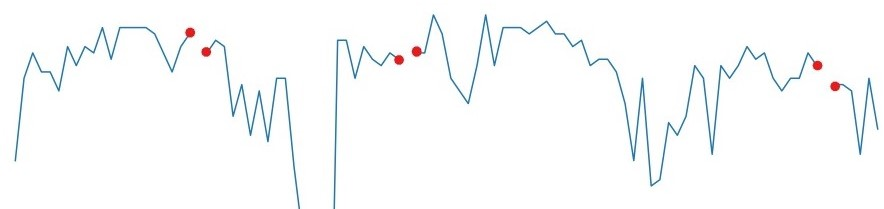
\includegraphics[width=0.7\textwidth]{img/extrapoalting.jpg}
\caption{the two ending non missing values of a gap}
\label{fig:extrapo}
\end{figure}

Yet another type of architecture we did not study in this project is Non-Autoregressive, since  autoregressive models  suffer from error propagation which becomes catastrophic for imputing long-range sequences, instead we can use  deep generative models. as in the following paper that was published on may 2019 under the name NAOMI: Non-Autoregressive Multiresolution
Sequence Imputation. \cite{naomi}.




\section{Acknowldgement}

We'd like to express our gratitude to our supervisor, Bertand Leger, for his guidance  throughout our research and shared with us his vast knowledge and
experience in the fields of internet of things and machine learning.

Also i would like to thank   '' la Direction Interdépartementale des Routes Est (DIR Est) for giving us access to their traffic database which. 


